\documentclass[conference]{IEEEtran}

\IEEEoverridecommandlockouts

\newcommand{\squeezeup}{\vspace{-2.5mm}}
\usepackage{array}
\newcolumntype{C}[1]{>{\centering\arraybackslash}m{#1}}
\usepackage{makecell}
\usepackage{cite}
\usepackage{hyperref}
\hypersetup{
	colorlinks=false,
	pdfborder={0 0 0},
}
\usepackage[pdftex]{graphicx}
\usepackage{url}
\usepackage{soul}
% correct bad hyphenation
\hyphenation{op-tical net-works semi-conduc-tor}

%table
\usepackage{tabularx}
\newcolumntype{L}{>{\raggedright\arraybackslash}X}
\usepackage{multirow}

%graph
\usepackage{siunitx}
\usepackage{tikz} % To generate the plot from csv
\usepackage{pgfplots}
\pgfplotsset{compat=1.12}
\pgfplotsset{compat=newest} % Allows to place the legend below plot
\usepgfplotslibrary{units}

\usepackage{listings}
\usepackage{fancyvrb}
\usepackage{framed}
\usepackage[listings,skins]{tcolorbox}
\usepackage[skipbelow=\topskip,skipabove=\topskip]{mdframed}
\mdfsetup{roundcorner=0}

\usepackage[colorinlistoftodos]{todonotes}

\lstset{
	basicstyle=\footnotesize\tt,        % the size of the fonts that are used for the code
	breakatwhitespace=false,         % sets if automatic breaks should only happen at whitespace
	breaklines=true,                 % sets automatic line breaking
	captionpos=b,                    % sets the caption-position to bottom
	extendedchars=true,              % lets you use non-ASCII characters; for 8-bits encodings only, does not work with UTF-8
	frame=single,                    % adds a frame around the code
	language=Java,                 % the language of the code
	keywordstyle=\bf,
	showspaces=false,                % show spaces everywhere adding particular underscores; it overrides 'showstringspaces'
	showstringspaces=false,          % underline spaces within strings only
	showtabs=false,                  % show tabs within strings adding particular underscores
	tabsize=2                       % sets default tabsize to 2 spaces
}

\usepackage{textcomp}

\renewcommand\IEEEkeywordsname{Keywords}

% table caption
\usepackage{xpatch}
\makeatletter
\patchcmd\@makecaption{\\}{.~}{}{\fail}
\makeatletter
\raggedbottom
\begin{document}

\title{AI-XAI-LLM: Interpretable Insights \\into Stroke Risk Prediction}

\author{
\IEEEauthorblockN{Thilini Bhagya}
\IEEEauthorblockA{
\textit{Lincoln University}\\
Lincoln, New Zealand\\
thilini.bhagya@lincoln.ac.nz
}
\and
\IEEEauthorblockN{Vindya Senanayake, Tharindu Thilakarathna,\\ Sanjaya Samudra, Gilmini Geethika}
\IEEEauthorblockA{
\textit{University of Sri Jayewardenepura}\\
Nugegoda, Sri Lanka\\
\{vindya, fc115538, fc115634, gilmini\}@sjp.ac.lk
}
}

\IEEEoverridecommandlockouts
\IEEEpubid{\makebox[\columnwidth]{979-8-3315-5723-2/26/\$31.00 \copyright2026 IEEE \hfill} \hspace{\columnsep}\makebox[\columnwidth]{ }}
\maketitle

\begin{abstract}
Early identification of individuals at stroke risk is critical for implementing timely preventive measures. Although machine learning models have demonstrated potential in predicting stroke risk, their clinical adoption is limited due to a lack of transparency. Explainable AI (XAI) techniques provide insights into predictions, but their technical metrics are often complex and difficult for clinicians to interpret. This research proposes an integrated AI-XAI-LLM pipeline that generates accurate, patient-specific stroke predictions and provides post-hoc explainability to highlight key factors influencing the prediction, which are then translated into clear, clinician-friendly narratives using a prompt-engineered large language model. Evaluations show that this approach enhances prediction transparency and interpretability, fostering trust and encouraging the use of predictions to support decision-making.
\end{abstract}

\medskip

\begin{IEEEkeywords}
\textit{explainability, LLM, SHAP, stroke prediction, XAI}
\end{IEEEkeywords}

\section{Introduction} \label{sec:introduction}
As a non-communicable disease, stroke is a leading cause of sudden death or long-term disability, and the second leading cause of death worldwide. According to statistics from~\cite{Feigin2025}, death rates due to cardiovascular diseases have increased considerably (with approximately 7 million deaths annually), emphasising the need for early identification of individuals at high risk. Early preventive measures, together with personalised treatment strategies are a proven path to reduce stroke risk and improve patient health conditions~\cite{dattani2023cardiovascular}.

\medskip 
Artificial Intelligence (AI), particularly Machine Learning (ML) and Deep Learning (DL), has attracted growing interest in the development of early diagnostic mechanisms in non-communicable diseases, working as decision assistance, supporting medical professionals in diagnosis and decision-making processes~\cite{alowais2023revolutionizing, davenport2019potential}. Stroke risk prediction has emerged as a key application area, where classical ML algorithms have been applied for structured electronic health records and DL methods for complex, unstructured data (including medical images and biosignals). However, the lack of transparency in many AI solutions (which are \textit{black-box} to users, meaning they can only observe the output but not how the internal structure works) remains a significant barrier to their clinical adoption. Epistemic transparency (i.e., clear understanding of how AI models arrived at their predictions) has therefore been recognised as a critical requirement for secure and reliable AI adoption in healthcare settings~\cite{winter2023troubling}. 

\medskip 
Explainable Artificial Intelligence (XAI) techniques, such as SHAP (SHapley Additive exPlanations)~\cite{lundberg2017unified} and LIME (Local Interpretable Model-agnostic Explanations)~\cite{ribeiro2016should}, have been introduced to address the opaque nature of AI models by providing insights into predictions. These methods are known as \textit{post-hoc interpretability} methods (applied after model training), offer both local explanations (interpret individual predictions by highlighting the key input features influencing each) and global explanations (provide overall understanding on how features affect the model)~\cite{samek2019towards}. In clinical applications (including stroke prediction), local interpretability is particularly important for understanding the key factors that lead a patient to be classified as at risk of stroke. Recent studies in stroke prediction have combined models with XAI (especially SHAP) in an effort to promote transparency, trust, and clinical acceptance of AI solutions~\cite{l7, lee2023interpretable, l8, l9, l15, l10, l11, l12, l23, l13, l14, l6}. Moreover, explainability is becoming a regulatory requirement as frameworks such as the General Data Protection Regulation (GDPR)\footnote{\url{https://gdpr-info.eu/} [accessed Nov. 23 2025]} mandate that clinicians to understand the medically relevant factors influencing AI predictions, even when these tools are used only for decision support. Despite this advancement, most XAI outputs (like those from SHAP) are typically quantitative and remain challenging for non-technical clinical professionals to interpret (understanding results need specialised knowledge in AI)~\cite{l6}. Although visualisations (e.g., Summary Plots, Dependence Plots) can help represent these values graphically, they often face similar challenges in effectively conveying the information. Large Language Models (LLMs) which are known for their strong language understanding and processing capabilities, generate context-aware human-readable output and have the potential to improve the interpretability of XAI outcomes~\cite{zeng2024enhancing}.


\medskip 
This study proposes integrating LLMs into the ML pipeline to transform XAI outputs into clear, clinician-friendly natural language explanations. For example, when a model predicts that a patient is at risk of stroke, the LLM translates the XAI output into a narrative outlining the key factors impacting the prediction. This integration connects individual predictions with meaningful clinical factors, allowing experts to better understand the rationale behind stroke risk predictions, validate the outputs, and ultimately accept or reject them. While integrating LLMs into clinical workflows raises valid concerns regarding data sensitivity, our approach mitigates these risks by using only anonymised input (e.g., feature-level values and feature importance scores), thereby avoiding the exposure of any patient identity data.

\medskip
Accordingly, the goal of this research is to design and evaluate an integrated AI-XAI-LLM pipeline that not only predicts stroke risk accurately, but also generates interpretable insights into the key features influencing these predictions to support comprehension of the model outcomes. To the best of our knowledge, this research represents one of the earliest efforts in healthcare to integrate LLMs for interpreting XAI outputs and generating clinician-friendly explanations, thereby advancing transparency in medical decision support. We use the publicly available Stroke Prediction Dataset from Kaggle\footnote{\url{https://kaggle.com/datasets/fedesoriano/stroke-prediction-dataset} [accessed Nov. 23 2025]\label{fn:dataset}}, which is widely recognised as a benchmark for research in stroke risk prediction, and employ Random Forest classifier~\cite{breiman2001random} given its proven performance in previous studies using the same dataset. 

\section{Literature Review} \label{sec:review}
ML has become a powerful tool for assessing stroke risk. Comparative studies~\cite{islam2021stroke, tazin2021stroke} have evaluated traditional ML algorithms in stroke prediction, such as Logistic Regression (LR), Decision Trees (DT), K-Nearest Neighbours (K-NN), and Random Forest (RF), using the Kaggle Stroke Prediction dataset. These studies demonstrated RF as the top-performing classifier. Another study~\cite{dev2022predictive} conducted on the same dataset demonstrated that Neural Networks (NN), particularly when trained with key features like age, heart disease, average glucose level, and hypertension, achieved the best performance compared to classical methods. Ensemble and hybrid models have also been investigated for their ability to improve performance. For example, one approach~\cite{l1} used a Dense Stacking Ensemble with RF as the meta-classifier, demonstrating the potential of stack-based ensembles for accurate prediction on the Kaggle dataset. A subsequent study~\cite{l2} combined RF and DT as base classifiers with LR as the meta-classifier, while another study~\cite{l3} improved model performance by combining RF and LR. Though these approaches have marked successes, challenges remain, especially as models lack comprehension.

\medskip
To improve the transparency of ML models, researchers have started integrating XAI techniques into stroke risk prediction, with SHAP being the popular choice to identify influential factors both at global and local levels. For example, one study~\cite{l7} demonstrated the use of DL alongside classic ML algorithms on a local dataset, showing that a simpler RF model was more reliable than a deep NN, and used SHAP to understand features contributed most. Another study~\cite{lee2023interpretable} used an eXtreme Gradient Boosting model for acute ischemic stroke prediction, applying SHAP at both global and instance levels. A related study~\cite{l8} developed an ensemble model using both a local dataset and the Kaggle dataset, incorporating SHAP and LIME to interpret individual predictions. Similarly, one approach~\cite{l9} introduced a shallow NN that outperformed standard classifiers, combining LIME with SHAP to provide instance level factors, while another study~\cite{l15} also employed SHAP and LIME in related tasks. Additionally, two studies~\cite{l10, l11} used an internally sourced dataset to address ischemic stroke prognosis supported by SHAP analysis, predicting one-year mortality with LR performing best and 90-day functional prognosis using SVM, respectively. A separate study~\cite{l12} validated top predictors using SHAP, LIME, and ELI5, while a subsequent study~\cite{l23} proposed an explainable ML pipeline evaluated on Kaggle data with interpretations via SHAP. Moreover, one study~\cite{l13} applied SHAP to interpret EMG-based post-stroke gait analyses, and another~\cite{l14} leveraged SHAP and ELI5 for EEG-based stroke prediction. However, these studies still need to be clinically validated in order to verify their relevance and accuracy. While the current level of interpretability enhances confidence in ML models to some degree, such abstract outputs remain largely numerical and are not readily understandable by non-AI experts, particularly medical professionals~\cite{l6}.

\medskip
Given the growing application of LLMs, recent studies in stroke prediction and management have highlighted the emerging role of LLMs in supporting
decision making. For example, one study~\cite{l20} designed
a domain-specific LLM by using clinical text and noncontrast
computed tomography (NCCT) for acute stroke diagnosis. Another approach~\cite{sarabadani2025skg} integrated LLMs with knowledge graphs to support stroke prognostics and personalised assessment. Furthermore,
hybrid AI architectures that combine traditional ML with LLMs
have been proposed to improve explainability as in~\cite{l22}. Recent work~\cite{l17} also evaluated the performance of LLMs for stroke prevention, diagnosis, and treatment.

\medskip
Although research on integrating XAI with LLMs is still in its early stages, recent studies in some domains provide promising evidence. In learning analytics, one framework~\cite{swamy2024explanations} combined XAI with LLMs to generate user-friendly explanations for critical features derived from students' online engagement patterns. Similar approaches have been applied in network intrusion detection\cite{khediri2024enhancing} and anomaly detection\cite{mekrache2024combining}. However, leveraging LLMs to interpret XAI outputs specifically in healthcare settings, including stroke prediction, remains largely unexplored. To address this gap, our research examines the integration of XAI and LLM technologies for stroke risk prediction.

\section{Methodology} \label{sec:methodology}
Fig.~\ref{fig:pipeline} depicts a high-level overview of the AI-XAI-LLM pipeline.
\begin{figure}[htbp]
\centerline{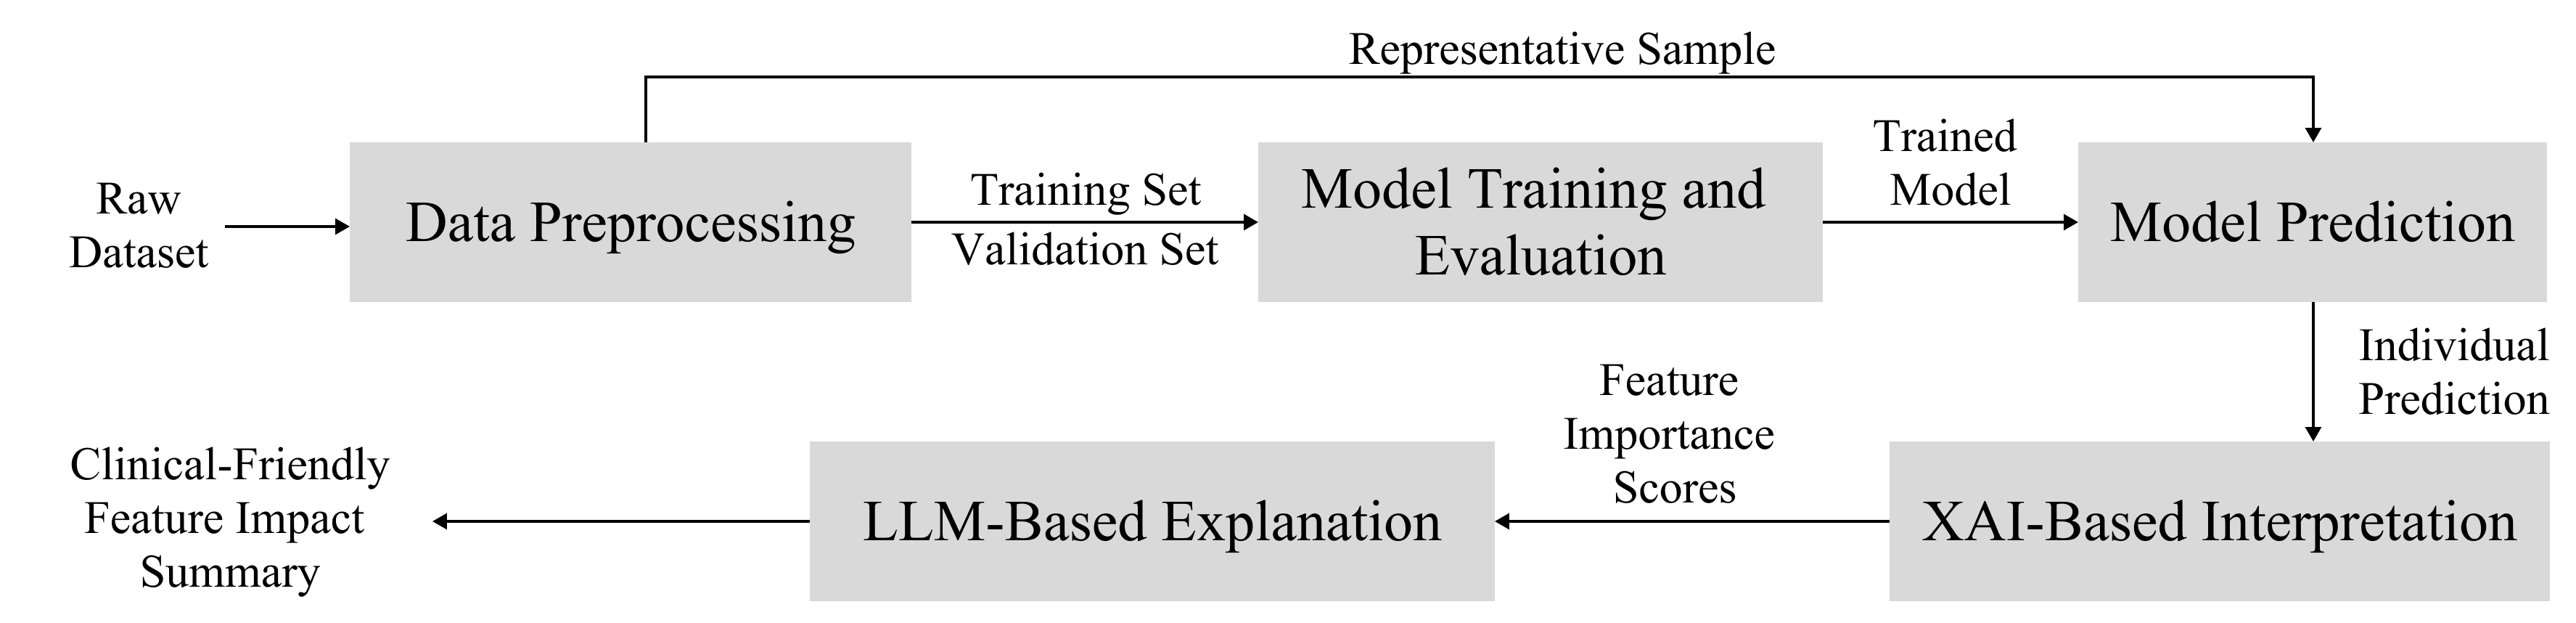
\includegraphics[width=\columnwidth]{graph-1}}
\caption{The AI-XAI-LLM pipeline}
\label{fig:pipeline}
\end{figure}
~\textbf{Data Preprocessing} is the initial phase that involves exploratory data analysis to understand the dataset, followed by cleaning and transformation steps to prepare the data for ML. The dataset is then split into a representative sample, and training/validation sets. In the~\textbf{Model Training and Evaluation} phase, the model is trained on the training set and evaluated on the validation set. The trained model is subsequently used in the~\textbf{Model Prediction} phase to predict outcomes for the representative sample. Following that, the~\textbf{XAI-Based Interpretation} phase uses XAI techniques to interpret each prediction by identifying key features driving the outcome. Finally, in the~\textbf{LLM-Based Explanation} phase, the LLM transforms the XAI outputs into clinician-friendly explanations, allowing users to easily comprehend the rationale behind the prediction. The fully reproducible pipeline can be accessed at: https://github.com/tbhagya/med-ai-xai-llm. The experiments were conducted using Python (version 3.11.2) on a computer with an Intel Core i5 processor and 16 GB RAM. Throughout the project, we engaged with a panel of seven medical officers (from Sri Lanka) and three general practitioners (from New Zealand) to familiarise ourselves with the domain, guide design decisions, and evaluate the final results.

\subsection{Data Preprocessing}
The dataset\textsuperscript{\ref{fn:dataset}} used in this research contains 5,110 patient records, each described by ten clinical and demographic information (i.e., \textit{gender}, \textit{bmi}, \textit{age}, \textit{hypertension}, \textit{heart\_disease}, \textit{ever\_married}, \textit{work\_type}, \textit{Residence\_type}, \textit{avg\_glucose\_level},  \textit{smoking\_status}), with the target (class) indicating if the patient had a stroke. From an ML perspective, this is a binary classification task that aims to classify patients into at stroke risk (1) or not at risk (0).

\medskip 
The target class is highly imbalanced, with only 249 stroke cases (4.87\%) compared to 4,861 non-stroke cases (95.13\%). Additionally, \textit{bmi}, \textit{age}, and \textit{avg\_glucose\_level} contained outliers; removing these would eliminate 113 stroke cases. Following consultation with clinical experts, these outliers were retained as they likely represent valid but rare cases (strokes are inherently rare, and outlier values may still hold clinical validity). For feature encoding, categorical variables (\textit{gender}, \textit{ever\_married}, \textit{work\_type}, \textit{Residence\_type}, and \textit{smoking\_status}) were transformed into numeric values using ordinal encoding (mapping each category to a unique integer). Moreover, \textit{bmi} contained 201 missing values. To impute these, we calculated absolute Pearson correlation coefficients between \textit{bmi} and other features, selecting only features with coefficients exceeding 0.2 as predictors. K-NN imputation was then applied (providing context-aware imputation rather than simply using mean or median values). 

\medskip
We set aside a representative sample of 15 patients (5 stroke and 10 non-stroke cases, maintaining class proportions) from the processed dataset, making sure that the selection captured feature diversity across key clinical variables. The remaining was used for model training and validation. To address the class imbalance, the Synthetic Minority Oversampling Technique (SMOTE)~\cite{chawla2002smote} was applied to oversample the minority (stroke) class, achieving a 1:1 ratio. While this can introduce optimistic bias, the objective was to train a generalised model capturing sufficient patterns from both classes. Continuous features (i.e., \textit{bmi}, \textit{age}, and \textit{avg\_glucose\_level}) were normalised using z-score normalisation to standardise input.

\subsection{Model Development}
In this research, we chose to use a classification algorithm that is well-established and proven to produce the best results in stroke prediction tasks. The Random Forest (RF) algorithm~\cite{breiman2001random} was selected accordingly. RF is a supervised ML algorithm that builds an ensemble of multiple decision trees using randomly selected subsets of data and features, with final predictions determined by majority vote. This randomisation helps avoid overfitting, making it especially suitable for medical data, which is typically complex, diverse, noisy, and imbalanced.

\medskip
Hyperparameter tuning was conducted using grid search with 5-fold cross-validation on the SMOTE-balanced training data, identifying optimal settings: 400 trees, maximum depth of 20, 1 minimum sample per leaf, 2 minimum samples per split, and square root of total features. The model was then retrained with these parameters. The performance was assessed using 5-fold cross-validation (to evaluate generalisability on unseen data). The metrics calculated include predictive accuracy (measures overall correctness on detecting stroke and non-stroke cases), recall (how well the model identify true stroke cases), precision (proportion of patients predicted to have a stroke who actually experienced one), F1-score (balanced metric that considers both precision and recall), and AUC-ROC (model's ability to distinguish between stroke and non-stroke cases). The average and standard deviation were reported for each to provide insights into the model's overall performance, stability, and variability. The trained model then predicted stroke status for individual patients in the representative sample.

\subsection{XAI for Instance-Level Interpretation}
Following individual predictions, focus shifted to generating local explanations for each case. In this research, SHAP~\cite{lundberg2017unified} was used as the local post-hoc XAI method. SHAP is currently recognised as the state-of-the-art in XAI~\cite{l6} and has demonstrated better results in stroke prediction research compared to other techniques. SHAP uses Shapley values (from game theory) to measure importance of each input feature, with positive or negative values indicating its effect on increasing or decreasing a prediction. These quantitative values are translated into human-readable explanations in the subsequent phase.

\subsection{LLM Integration}
We employed LM Studio\footnote{\url{https://lmstudio.ai/} [accessed Nov. 23 2025]}, which is a widely adopted desktop platform that supports running most LLMs from Hugging Face. It operates by deploying a local server accessible with a RESTful API, allowing straightforward integration with any programming environment. Given the increasing capabilities of open-source LLMs, we selected the Gemma model (i.e., gemma-3n-e4b)\footnote{\url{https://huggingface.co/google/gemma-3n-E4B} [accessed Nov. 23 2025]}, which is publicly and freely available on Hugging Face and supported by LM Studio. Gemma is inspired by Google's Gemini frontier model and is relatively lightweight  (approximately 4.24GB on disk), making it well suited for our setup. However, to promote extensibility and support alternative LLMs, we implemented a generic wrapper function based on OpenAI API standards.

\medskip
We explicitly selected the top three positive SHAP values to generate clear, clinician-friendly narrative explanations. This approach highlights only the most influential factors for prediction, while excluding less impactful contributors. It enhances clarity, aligns with clinical preferences for concise and straightforward information, and is consistent with prior work on interpretable clinical ML. To improve interpretability and to consistent with medical reporting standards, feature names were mapped to standardised clinical terms (e.g., \textit{bmi} to \textit{Body Mass Index}, \textit{hypertension} to \textit{High Blood Pressure}), and binary values (in  \textit{hypertension}, \textit{heart\_disease}) were translated to \textit{Present} or \textit{Absent}. Continuous variables (such as \textit{bmi}, \textit{avg\_glucose\_level}) were formatted in standard clinical units (\textit{kg/m²} for \textit{bmi}, \textit{mg/dL} for \textit{avg\_glucose\_level}).

\medskip
Prompt engineering played a critical role to ensure LLM outputs are accurate, contextually relevant, and easy to understand in clinical settings. Developing the optimal prompt involved an iterative process of experiments and testing with various prompt structures and input formats. To validate and refine the prompts, we engaged with experts whose feedback guided successive prompt adjustments, significantly improving the clarity and applicability of the generated explanations. For prompt design, we followed the DAIR.AI Prompt Engineering Guide\footnote{\url{https://promptingguide.ai/} [accessed Nov. 23 2025]} and the methodology proposed by~\cite{zytek2024llms}. We selected a few-shot chain-of-thought (CoT) prompting technique, combining multiple structured examples with explicit, step-by-step clinical reasoning. This guides the LLM to generate incremental reasoning through each feature's contribution to stroke risk. Recent research in clinical prompt engineering demonstrates that few-shot CoT prompting optimises LLM performance in diagnostic support and explanation tasks, outperforming zero-shot or isolated few-shot methods~\cite{liu2025prompt}, which is supported by our experimental findings. The prompt includes a system-level instruction that defines the LLM's role as a clinical summarisation assistant specialised in stroke risk assessment. This is complemented by few-shot example narratives that demonstrate the expected explanation style, level of detail, and clinical terminology. The input to the prompt includes the patient's specific prediction, values of all relevant features, and the top three features most influential to the prediction as identified by SHAP values. The LLM output is set to include the predicted stroke risk, the patient's feature values, detailed yet concise clinician-style explanations for each of the top three influential features, and a final summary highlighting their combined impact. Furthermore, we fine-tuned the hyperparameters of the Gemma model to optimise explanation quality. Specifically, the temperature was set to 0.3 and top\_p  to 0.7 to encourage factual, concise responses. The max token length was limited to 150 tokens to avoid overly verbose outputs. 

\medskip
The same expert panel evaluated final explanations by comparing two presentation formats: stroke risk predictions with raw SHAP values (baseline) versus natural language explanations from our AI-XAI-LLM pipeline. Clinicians rated each case under both conditions on a 5-point Likert scale (1 = lowest, 5 = highest) using two criteria: Clarity (How clearly does the explanation communicate the key factors influencing the prediction?) and Trust (How much does the explanation increase your confidence in the prediction?). We calculated mean ratings and standard deviations per criterion, with statistical significance assessed via paired t-tests and inter-rater reliability via Krippendorff's alpha.

\section{Results and Discussion}
The model achieved an average predictive accuracy of 0.9576 ± 0.0028, with most cases correctly classified. Recall was notably high (0.9755 ± 0.0018), indicating the model's strong ability to correctly identify actual stroke cases (true positives) while lowering false negatives (stroke patients incorrectly predicted as not having a stroke). This demonstrates that the model is particularly reliable in detecting actual stroke cases, even if they are rare. The average precision of 0.9419 ± 0.0040 indicates that most predicted stroke cases were true positives, lowering false positives (patients incorrectly predicted as having a stroke). With an average F-Score of 0.9584 ± 0.0027, we can be reasonably confident that the model balanced false negatives and false positives. The AUC-ROC of 0.9937 ± 0.0009 confirms the competitive performance of the model in distinguishing stroke versus non-stroke cases. The consistently low standard deviations across all measures (0.0009 – 0.0040) confirm stable performance across all cross-validation folds. Overall, the model reliably and accurately identifies stroke patients while reducing false alarms. However, some borderline cases were not sufficiently captured in the dataset, potentially introducing instability in predictions.
\begin{figure}[!htbp]
\centering
\begin{tcolorbox}[
    colback=gray!5,        % light background
    colframe=gray!50,      % ash/gray border
    sharp corners,
    boxrule=0.2mm,         % thinner border
    fontupper=\ttfamily\footnotesize,
    left=1mm,
    right=1mm,
    boxsep=1mm,
    top=1mm,
    bottom=1mm
    ]
\textbf{Predicted Stroke Status}: Risk\\
\textbf{Patient Data}:\\
Sex: Male\\
Age: 81 years\\
High Blood Pressure: Present\\
Cardiovascular Disease History: Present\\
Marital History: Yes\\
Occupation Type: Government Job\\
Living Environment: Urban\\
Average Glucose Level: 250.9 mg/dL\\
Body Mass Index (BMI): 28.1 kg/m²\\
Smoking History: Smokes\\
\textbf{Explanation}: The input features that had the greatest impact on the stroke risk prediction were Age, Average Glucose Level, and Body Mass Index (BMI).\\
\textbf{Age}: The patient’s advanced age of 81 years is associated with increased cerebrovascular risk due to inherent vascular aging and increased susceptibility to stroke.\\
\textbf{Average Glucose Level}: A significantly elevated average glucose level of 250.9 mg/dL suggests impaired glucose metabolism, which can contribute to endothelial dysfunction and accelerate atherosclerosis, increasing stroke risk.\\
\textbf{Body Mass Index (BMI)}: The patient’s BMI of 28.1 kg/m² classifies as overweight, potentially contributing to increased cardiovascular risk factors such as hypertension and diabetes, further elevating stroke probability.\\
\textbf{Overall Summary}: Advanced age, impaired glucose control, and being overweight combine to increase the patient’s stroke risk.
\end{tcolorbox}
\caption{A sample of AI-XAI-LLM explanation for a patient.}
\label{graph-2}
\end{figure}


\medskip
The comparative evaluation revealed that LLM-generated explanations significantly outperformed the SHAP-only baseline across both criteria. Clarity scores were 4.70 ± 0.30 for our approach compared to 2.30 ± 0.70 for baseline, while Trust scores were 4.30 ± 0.40 compared to 2.10 ± 0.80. LLM-generated narratives clearly communicate the key factors influencing individual predictions, making them significantly easier to understand than raw SHAP values and allowing easy verification against clinical knowledge. Clinicians reported feeling more assured in deciding whether to trust and act on the predictions rather than merely wondering about the basis of the prediction or trying to interpret SHAP values and their influence on the outcome. Both differences were statistically significant (p $<$ 0.001), and inter-rater reliability was high for both (Krippendorff's $\alpha$ = 0.73 for baseline, $\alpha$ = 0.86 for our approach), indicating strong consistency across evaluations. Analysis across individual cases revealed variation in feature impacts, underscoring the need for transparent, individual-level explanations. Clinical factors such as age and glucose level were often strong predictors (consistent with clinical knowledge), while bmi showed more variable effects. Some demographic factors (e.g., occupation type, marital status, and residence) occasionally outweighed traditional clinical risk factors. Interestingly, hypertension and heart disease (although clinically critical) had minimal impact on many predictions, possibly because the dataset did not sufficiently capture their contribution. This discordance between model-identified features and clinical expectations is reflected in the LLM-generated explanation ratings, which, while significantly improved over SHAP-only presentations, did not achieve perfect scores. In cases where feature contributions appear clinically contradictory, clinicians can confidently disregard predictions and rely primarily on their own judgment. 

\medskip
For example, consider a patient for whom the model correctly predicted stroke risk. The corresponding SHAP values for the prediction were: Age (+0.1794), Average Glucose Level (+0.0969), Occupation Type (–0.0554), Body Mass Index (BMI) (+0.0289), Marital History (+0.0121), High Blood Pressure (–0.0118), Sex (+0.0113), Smoking History (+0.0100), Cardiovascular Disease History (–0.0025), and Living Environment (+0.0009). While these values provide insights into model internals, clinicians struggle to comprehend them directly. Fig.~\ref{graph-2} shows an example of the AI-XAI-LLM explanation. The output clearly highlights the three primary contributors to stroke risk in clinically meaningful terms. Advanced age has a major influence on stroke risk, consistent with clinical evidence. The elevated average glucose level was another key factor, indicating that the model recognises diabetes-related complications as significant contributors to stroke risk, aligning with clinical understanding. The other top contributor was overweight bmi, which is clinically linked to hypertension and diabetes, both of which indirectly increase stroke risk. This explanation is clear, natural, and sufficiently detailed, making it suitable for clinicians without AI expertise to understand. It demonstrates model transparency by explicitly showing the top features that influenced the final output, thus helping clinicians interpret and trust the prediction. However, hypertension and heart disease did not contribute to the stroke risk of this patient, reflecting a common limitation in the dataset.

\medskip
Overall, our results confirm the effectiveness and practicality of integrating XAI with LLM (through a specifically designed prompt) to generate patient-specific stroke risk explanations that are clinically interpretable. The AI-XAI-LLM pipeline can be adapted to other clinical prediction tasks with appropriate domain-specific modifications, and more generally to any domain where XAI outputs need to be made understandable for non-technical users.

\medskip
While the results demonstrate both strong predictive performance and improved interpretability, we acknowledge several limitations that may affect generalisability. First, both training and validation relied on a single public dataset, limiting applicability across diverse patient populations and clinical settings. However, this benchmark dataset contains sufficient clinical diversity for initial model development, and future work will validate/retrain the model on additional datasets featuring greater variety in patient demographics and clinical parameters. Second, the use of SMOTE for handling class imbalance may produce overly optimistic results. We are certain that applying it exclusively to training data, employing cross-validation for unbiased evaluation, and consulting clinical experts throughout to verify that results remained clinically realistic, mitigated this risk to a large extent. Third, the clinician evaluation panel was limited with a relatively small sample size. However, we ensured to follow a structured evaluation process and achieved high inter-rater reliability and statistically significant results.

\section{Conclusion} \label{sec:conclusion}
This research introduced an AI-XAI-LLM pipeline that improves the interpretability of stroke risk prediction by translating quantitative XAI outputs into clear, clinician-friendly explanations using LLM. Despite the dataset falls short in adequately covering edge cases, potential optimistic bias from class balancing, which impact model performance and generalisability, and the limited scope of clinical evaluation, the framework demonstrates strong potential to enhance stroke prediction. The pipeline could also be extended to broader medical applications and, more generally, to any domain requiring translation of technical XAI outputs into user-friendly explanations. Future work will include training the model on more comprehensive and diverse datasets, verifying explanations with multidisciplinary clinical cohorts, and assessing usability in real-world clinical settings. 

% references
\begingroup
\bibliographystyle{IEEEtran}
\def\IEEEbibitemsep{0pt plus .5pt}
\bibliography{bibliography}
\endgroup
	

\end{document}
